\documentclass{article}
% ── Author comment macros ────────────────────────────────────────────────────
\newcommand{\red}[1]{{\color{red}#1}}
\newcommand{\todo}[1]{{\color{red}#1}}
\newcommand{\TODO}[1]{\textbf{\color{red}[TODO: #1]}}
\newcommand{\mypar}[1]{\noindent\textbf{#1}}

\newcommand{\anis}[1]{{\color{magenta}{[AR] #1}}}
\newcommand{\einari}[1]{{\color{teal}{[EH] #1}}}
\newcommand{\mete}[1]{{\color{orange}{[MA] #1}}}
\newcommand{\samuli}[1]{{\color{blue}{[SJ] #1}}}

% ── Layout & typography ───────────────────────────────────────────────────────
\usepackage[letterpaper, top=0.75in, bottom=0.75in, left=0.75in, right=0.75in, columnsep=0.25in]{geometry}
\usepackage[protrusion=true,expansion=false]{microtype}

% ── Author affiliations ───────────────────────────────────────────────────────
\usepackage{authblk}
\usepackage{cuted}

% ── Tables ───────────────────────────────────────────────────────────────────
\usepackage{booktabs}
\usepackage{tabularx}
\usepackage{multirow}
\usepackage{adjustbox}

% ── Figures ──────────────────────────────────────────────────────────────────
\usepackage{float}
\usepackage{caption}
\usepackage{subcaption}

% ── References ───────────────────────────────────────────────────────────────
\usepackage{natbib}
\setcitestyle{numbers,square}

% ── Colours & links ──────────────────────────────────────────────────────────
\usepackage[table]{xcolor}
\usepackage[colorlinks=true, linkcolor=blue, urlcolor=cyan, citecolor=green]{hyperref}

\graphicspath{{../figures/}}
\renewcommand{\thefigure}{S\arabic{figure}}
\renewcommand{\thetable}{S\arabic{table}}

\title{\textbf{Supplementary Information}\\[2pt]
\large Host-Conditioned Spatial Structure of Canopy Mortality in Finland's Boreal Forests}
\date{}

\begin{document}
\maketitle
\vspace{-2em}

This Supplement records the software environment and random seeds (\S\ref{si:env}), the shape-feature
correlation structure (\S\ref{si:corr}) and univariate feature AUCs (\S\ref{si:auc}) that underpin the
morphological-gradient framing, the per-figure provenance trail (\S\ref{si:prov}), and a set of
supporting figures relocated from the main text (\S\ref{si:figs}). It accompanies
the main text and uses the same cluster table (14,582 clusters; 3,422 elongated/dispersed ``Type\,0''
and 11,160 compact/aggregated ``Type\,1'').

% ============================================================================
\section{Software environment and random seeds}
\label{si:env}

\begin{table}[h]
\centering
\small
\begin{tabular}{@{}ll@{}}
\toprule
\textbf{Component} & \textbf{Version / value} \\
\midrule
Python              & 3.9.6 \\
\quad numpy / scipy & 2.0.2 / 1.13.1 \\
\quad pandas / scikit-learn & 2.3.3 / 1.6.1 \\
\quad geopandas / shapely / pyproj & 1.0.1 / 2.0.7 / 3.6.1 \\
\quad rasterio / pointpats & 1.4.3 / 2.3.0 \\
\quad matplotlib & 3.9.4 \\
R                   & 4.6.1 \\
\quad spatstat (.geom/.explore) & 3.6.1 (3.8.1) \\
\midrule
Covariance-preserving null seed & 42 \\
Discreteness tests (GMM/PCA) seed & 42 \\
Tree-level subsample seed & 42 \\
\texttt{spatstat} envelopes & 39 sims/block \\
DBSCAN \texttt{eps} (clusters / blocks) & 20\,m / 15\,km \\
DBSCAN \texttt{min\_samples} & 1 (deterministic) \\
Host/species raster vintage & MS-NFI \texttt{vmi1x\_1721} (2021) \\
\bottomrule
\end{tabular}
\caption{Software versions and seeds for full reproducibility. All stochastic steps are seeded;
DBSCAN is deterministic at \texttt{min\_samples}\,=\,1.}
\label{tab:si-env}
\end{table}

% ============================================================================
\section{Shape-feature correlation structure}
\label{si:corr}

The morphological features are strongly intercorrelated (Figure~\ref{fig:si-corr}). Aspect ratio and
elongation are effectively the same axis ($\rho=1.00$); compactness is its near-perfect inverse
($\rho=-0.85$); area, perimeter, core:edge ratio and point count form a tight size block
($\rho\ge0.71$). The three features used to define the $k=2$ partition (fractal dimension,
Clark--Evans, aspect ratio; red boxes) therefore span only two largely independent directions, an
elongation axis and a size/density axis, which is why a single principal component captures 60\% of
the variance (main text, \S Morphological Gradient) and why the partition is best read as a cut
through a continuum rather than two natural classes.

\begin{figure}[h]
  \centering
  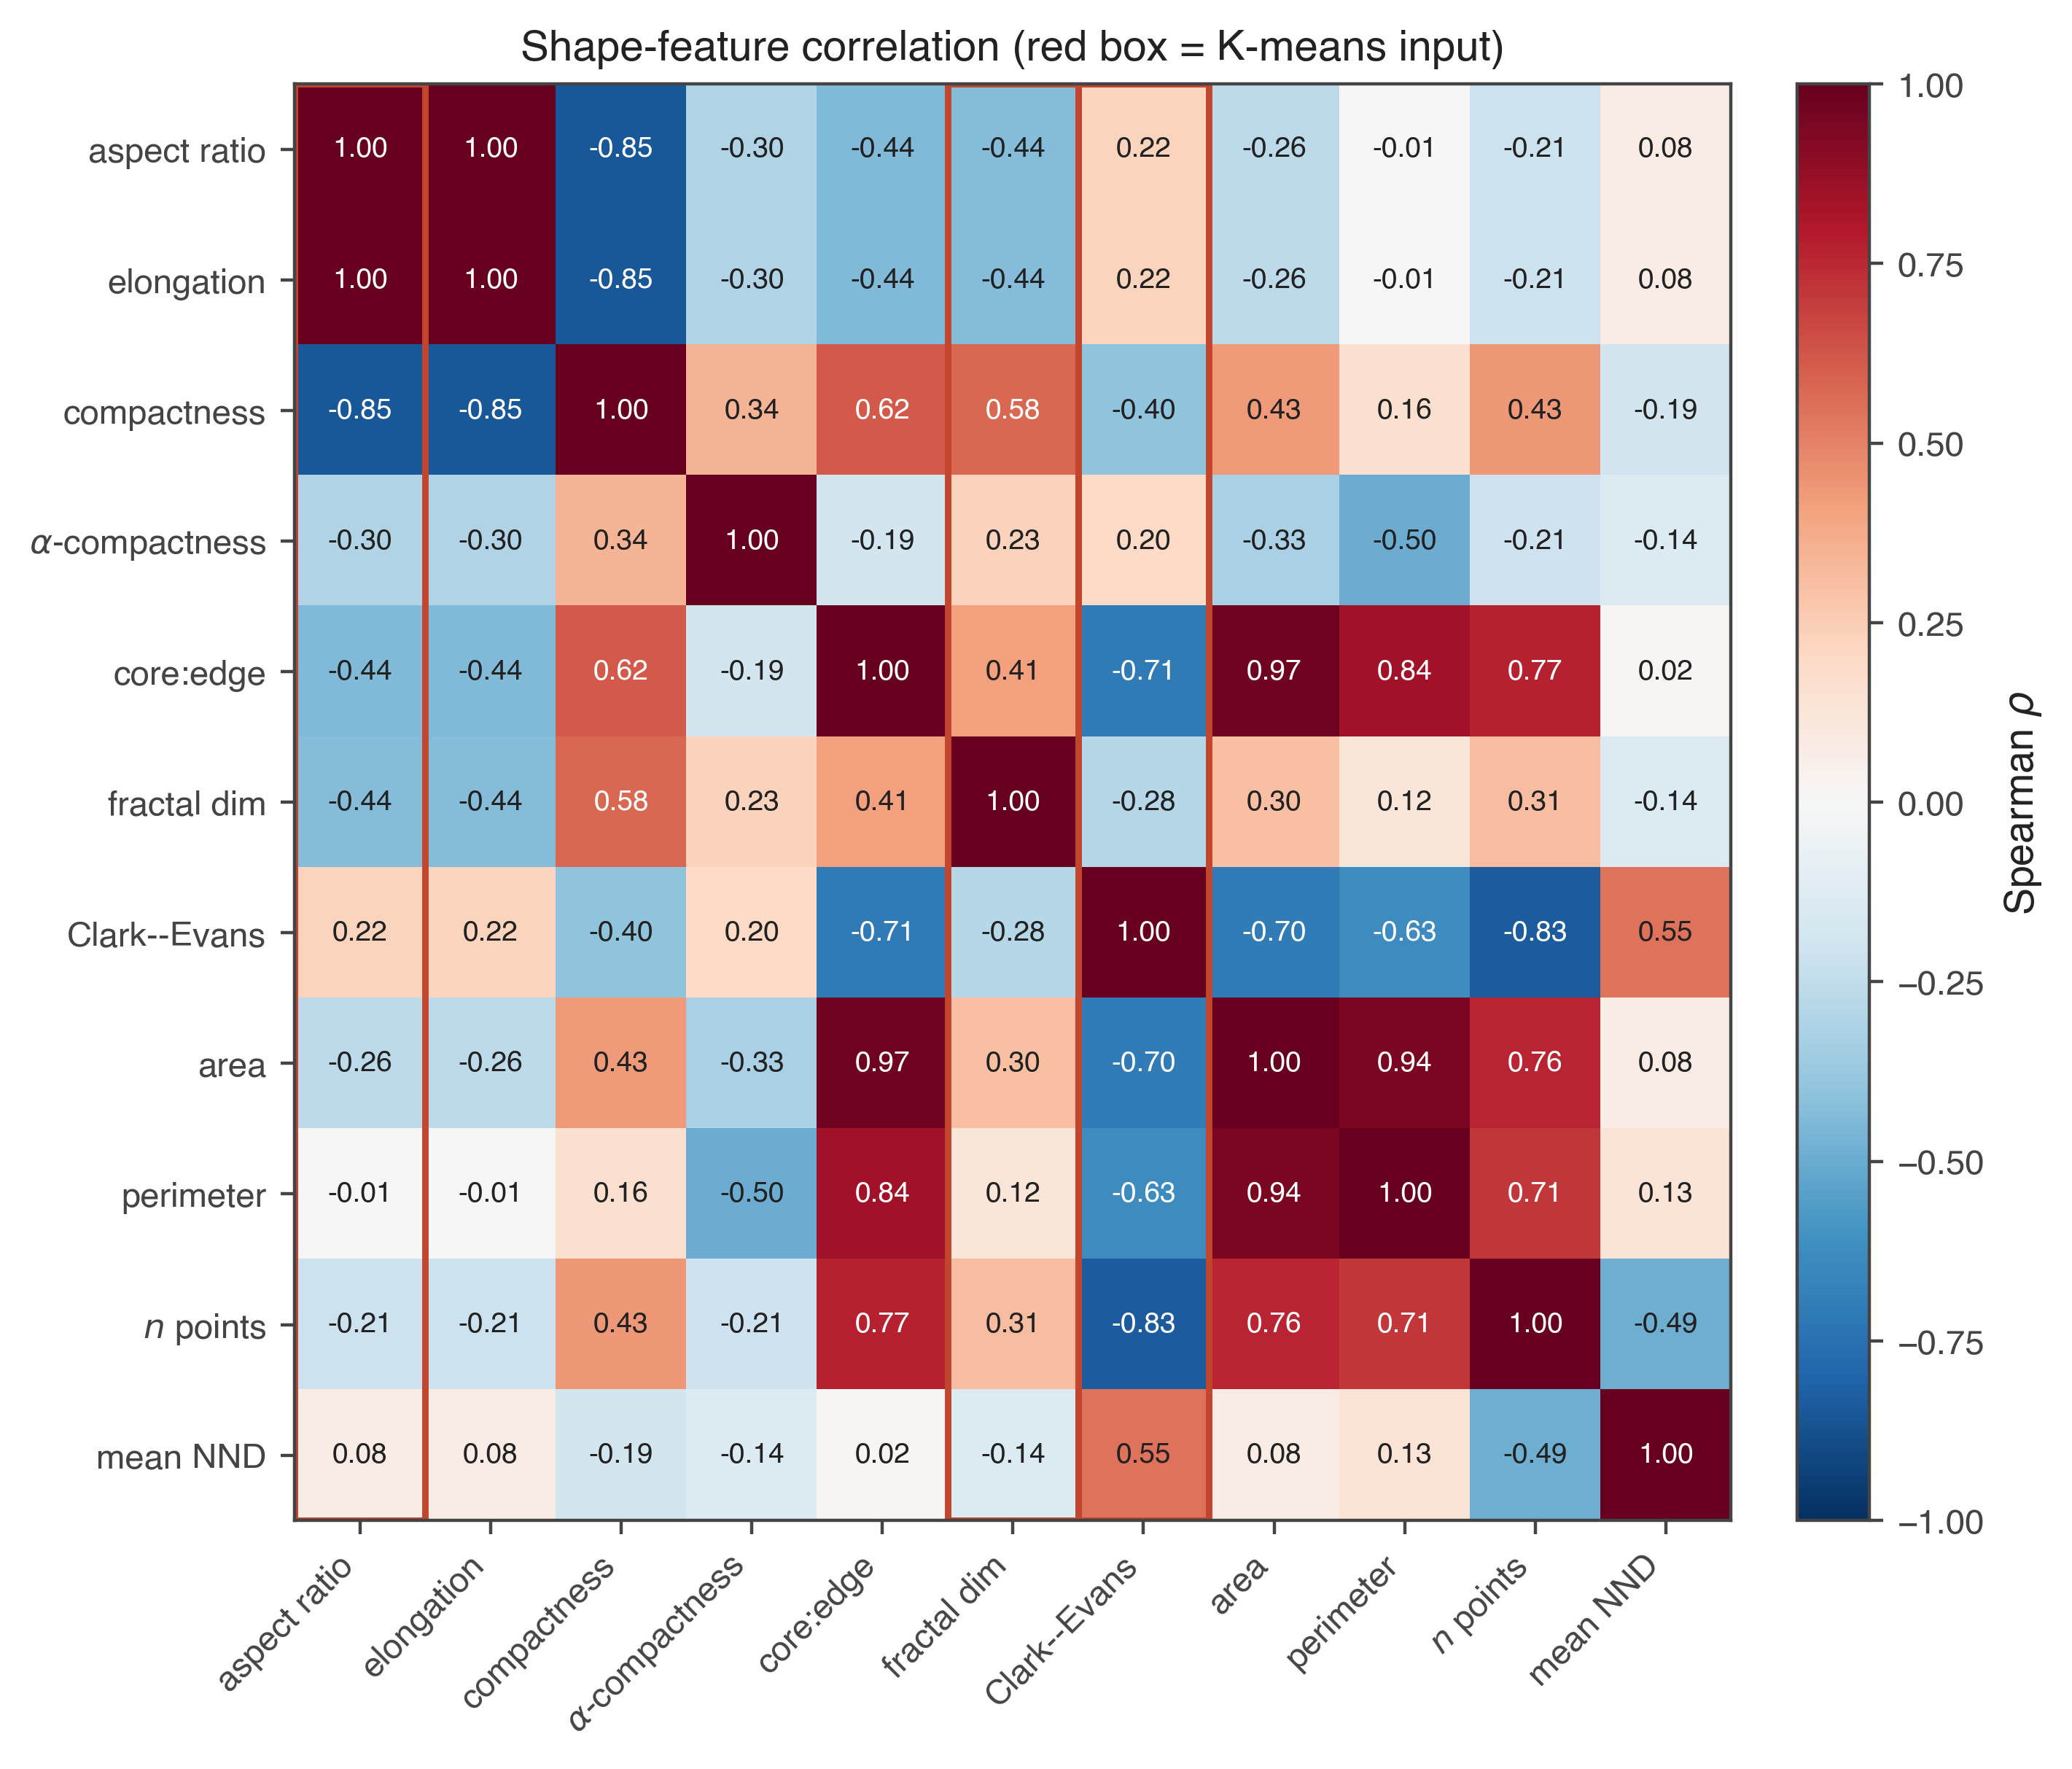
\includegraphics[width=\linewidth]{fig_si_corr.png}
  \caption{Spearman correlation among the eleven cluster-level shape and point-pattern features.
           Red boxes mark the three features input to $k=2$ K-means.}
  \label{fig:si-corr}
\end{figure}

% ============================================================================
\section{Univariate feature separability}
\label{si:auc}

Table~\ref{tab:si-auc} reports the area under the ROC curve for each feature taken alone as a
classifier of the two morphological endpoints (direction: ``$+$'' = larger values associate with the
compact endpoint). The high AUCs of compactness (0.961), aspect ratio (0.945) and elongation (0.945)
are \emph{expected and partly circular}: the partition is defined on aspect ratio and fractal
dimension, so any feature coupled to those axes separates the endpoints almost perfectly by
construction. These values quantify the geometric redundancy among descriptors discussed in the main
text; they are not independent evidence for two classes. The one shape-orthogonal quantity examined in
the main text, landscape connectivity, adds no separating signal once size is accounted for.

\begin{table}[h]
\centering
\small
\begin{tabular}{@{}lcc@{}}
\toprule
\textbf{Feature} & \textbf{AUC} & \textbf{Dir.\ (compact)} \\
\midrule
compactness & 0.961 & $+$ \\
aspect ratio$^\dagger$ & 0.945 & $-$ \\
elongation & 0.945 & $-$ \\
fractal dim$^\dagger$ & 0.938 & $+$ \\
core:edge & 0.837 & $+$ \\
Clark--Evans$^\dagger$ & 0.760 & $-$ \\
area & 0.733 & $+$ \\
$n$ points & 0.726 & $+$ \\
$\alpha$-compactness & 0.662 & $+$ \\
mean NND & 0.622 & $-$ \\
perimeter & 0.577 & $+$ \\
\bottomrule
\end{tabular}
\caption{Univariate ROC-AUC for separating the elongated (Type\,0) from the compact (Type\,1)
endpoint. $^\dagger$ = feature used to define the $k=2$ partition. Direction ``$+$'' = larger values
associate with the compact endpoint. High AUCs reflect geometric redundancy, not independent
validation.}
\label{tab:si-auc}
\end{table}

% ============================================================================
\section{Per-figure provenance}
\label{si:prov}

Every main-text figure is regenerated by a script in the public repository
(\url{https://github.com/aniskhan25/TreeMortSpatial}, \texttt{analysis/}); the \texttt{restyle\_*}
scripts apply the shared house style (\texttt{analysis/figstyle.py}) to notebook-produced figures.

\begin{table}[h]
\centering
\small
\begin{tabular}{@{}lll@{}}
\toprule
\textbf{Figure} & \textbf{Generating script} & \textbf{Primary input} \\
\midrule
fig2\_histograms & \texttt{make\_histograms\_figure.py} & cluster table \\
fig4\_scatters & \texttt{restyle\_charts.py} & cluster table \\
fig6\_typology\_map & \texttt{restyle\_maps.py} & cluster table \\
fig8\_local\_morans & \texttt{restyle\_maps.py} & \texttt{gate\_moran*} \\
fig\_shape\_space & \texttt{restyle\_charts.py} & cluster table \\
fig\_size\_dist & \texttt{restyle\_charts.py} & cluster table \\
fig\_orientation\_rose & \texttt{restyle\_charts.py} & cluster table \\
fig\_moran\_heatmap & \texttt{restyle\_charts.py} & \texttt{gate\_moran*} \\
fig\_silhouette\_permtest & \texttt{make\_permtest\_figure.py} & \texttt{discreteness\_tests.py} \\
fig\_dbscan\_sensitivity & \texttt{make\_gate\_figure.py} & \texttt{gate1\_eps\_stability} \\
fig\_anisotropy & \texttt{make\_anisotropy\_figure.py} & \texttt{gate3\_anisotropy} \\
fig\_shap\_heldout & \texttt{restyle\_shap.py} & held-out RF \\
fig\_contagion\_a/b & \texttt{restyle\_maps.py} & cluster table \\
fig\_sampling\_extent & \texttt{scope\_experiments.py} & cluster table \\
fig\_host\_conditioned & \texttt{make\_hostcond\_figure.py} & \texttt{host\_pointprocess.py} \\
fig\_hostcond\_rigor & \texttt{make\_hostcond\_rigor\_figure.py} & \texttt{linhom\_*.csv} \\
fig\_species\_validation & \texttt{species\_validation.py} & MS-NFI species rasters \\
fig\_si\_corr (this SI) & \texttt{make\_si\_tables.py} & cluster table \\
\bottomrule
\end{tabular}
\caption{Per-figure provenance. ``cluster table'' = \texttt{data/clusters\_typed.csv}; gate/host
artifacts are written to \texttt{analysis/out/}.}
\label{tab:si-prov}
\end{table}

% ============================================================================
\section{Supporting figures relocated from the main text}
\label{si:figs}

These descriptive and supporting figures are referenced from the main text. They were moved here to
keep the main figures focused on the three contributions; the analyses they depict are unchanged.

\begin{figure}[htb]
  \centering
  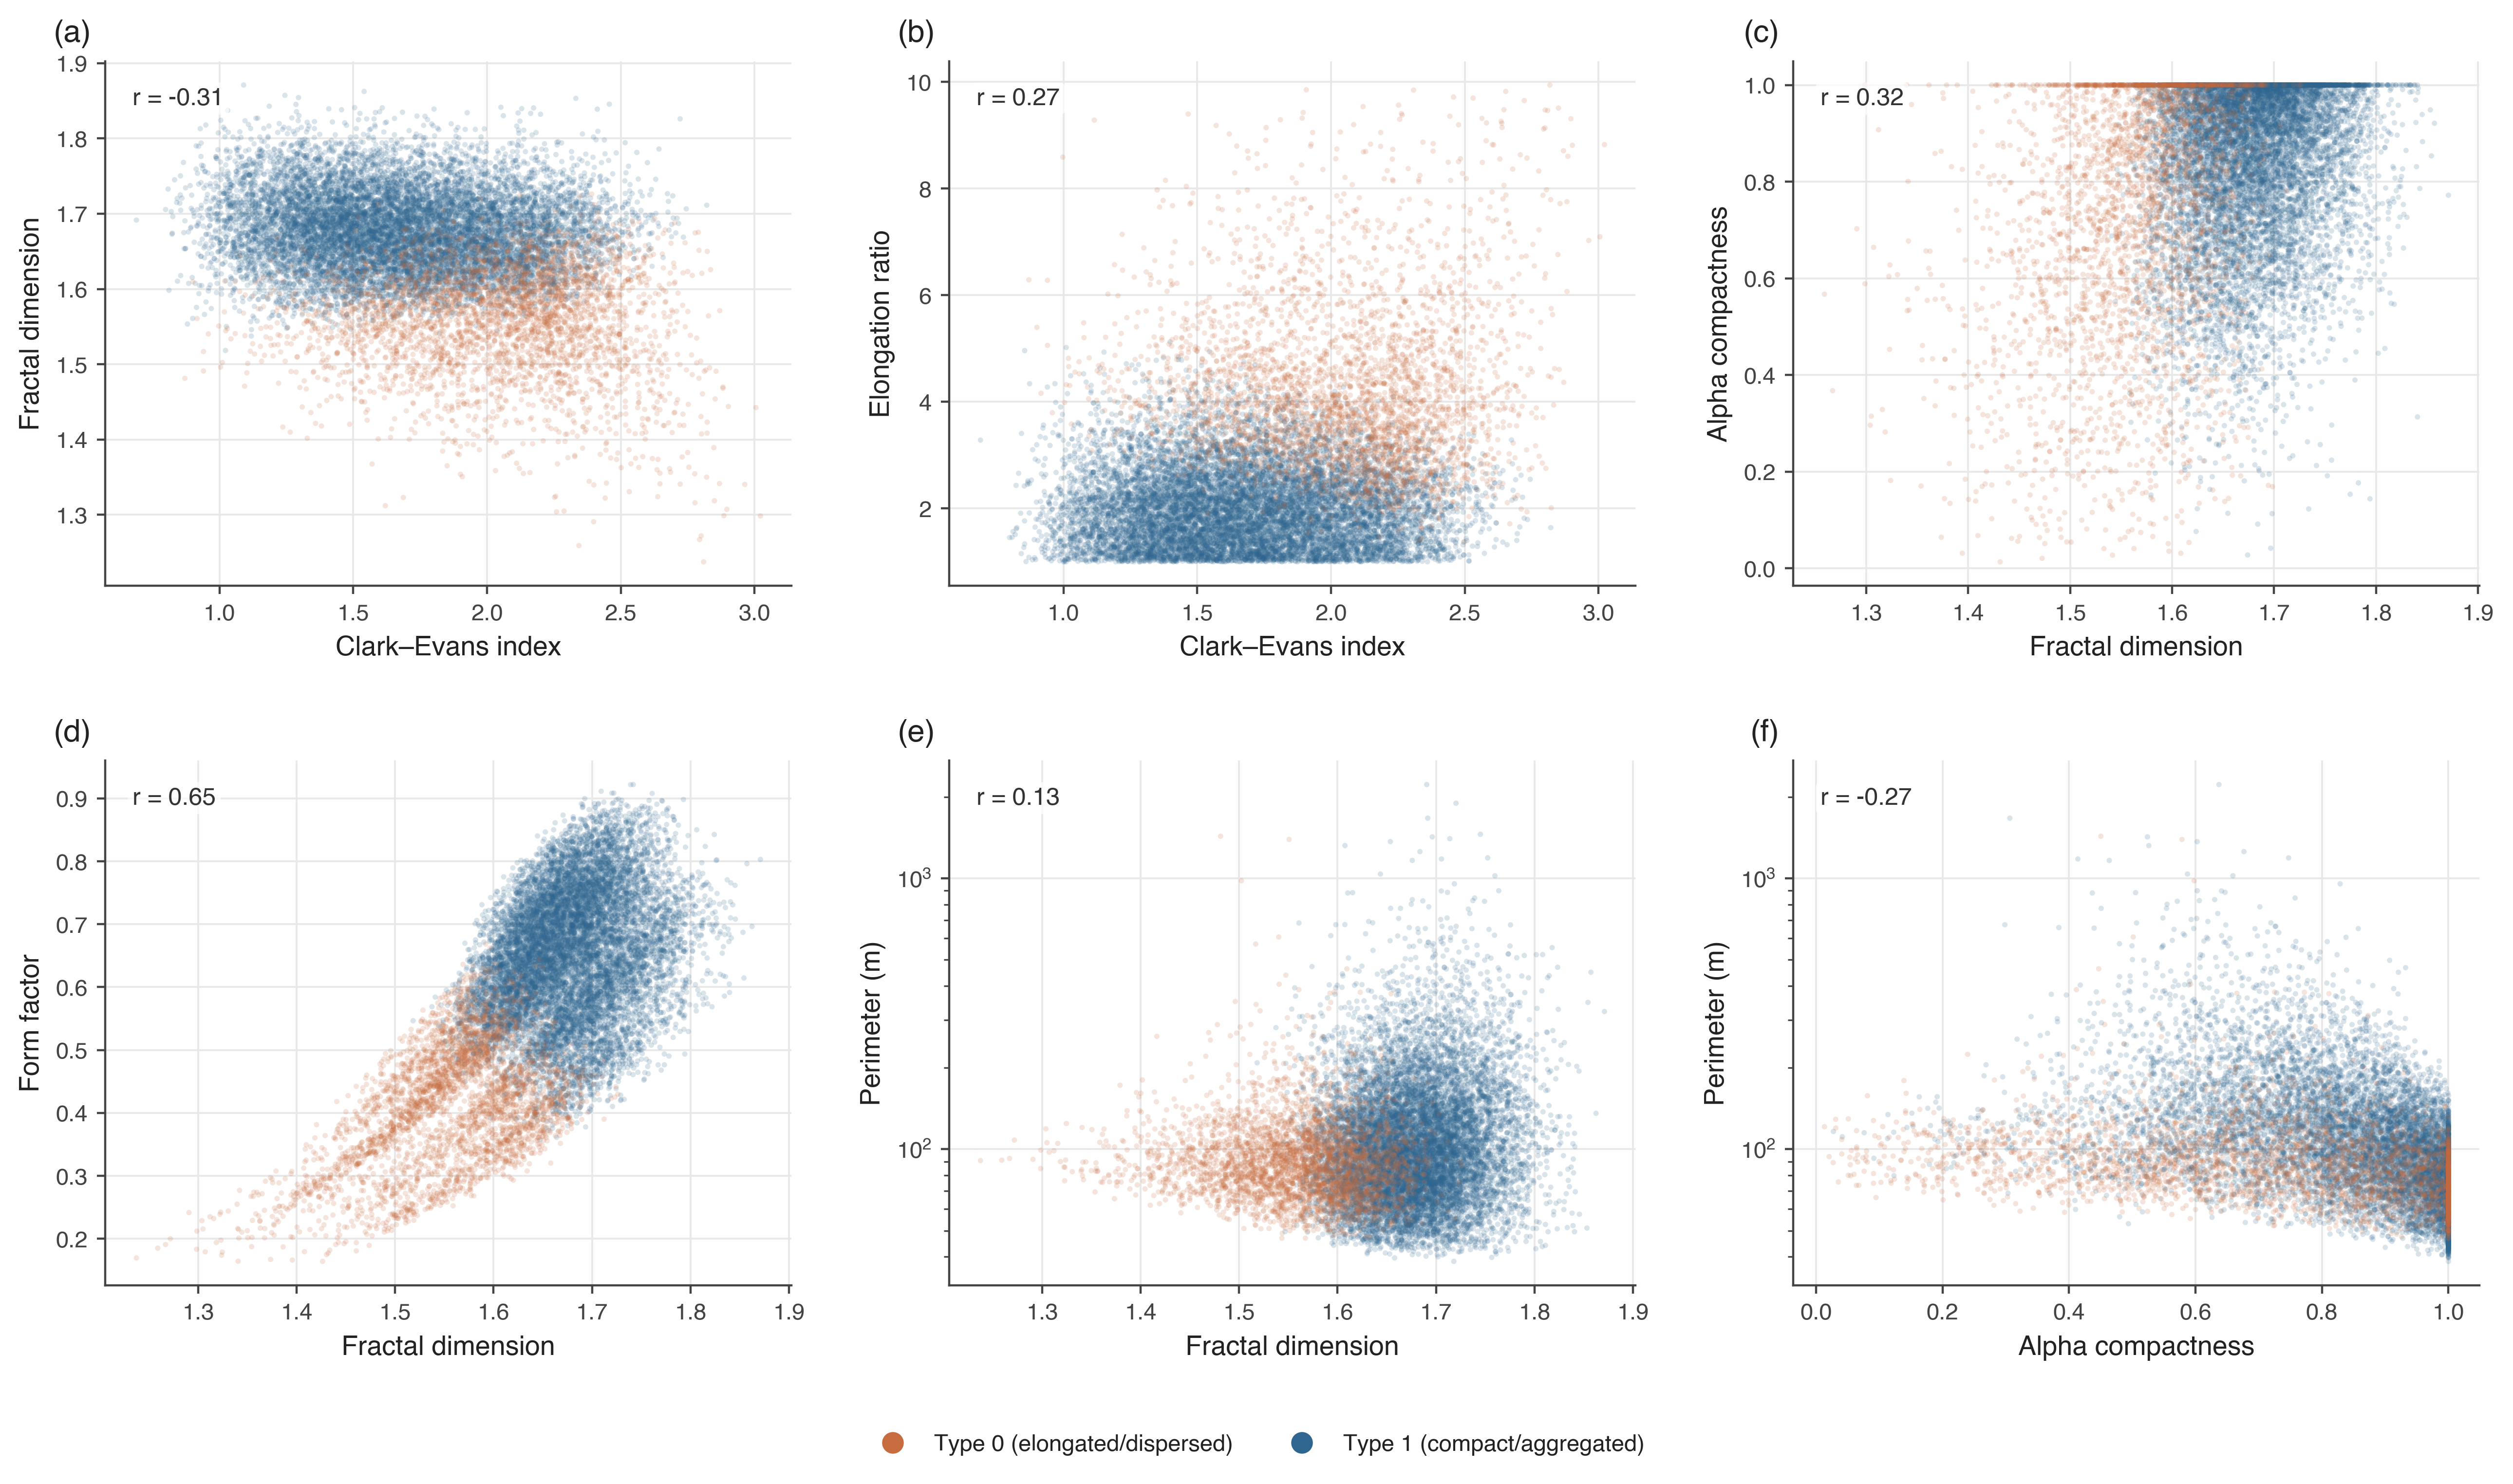
\includegraphics[width=0.9\linewidth]{fig4_scatters.png}
  \caption{Pairwise scatter plots of selected spatial metrics, coloured by morphological endpoint.}
  \label{fig:scatters}
\end{figure}

\begin{figure}[htb]
  \centering
  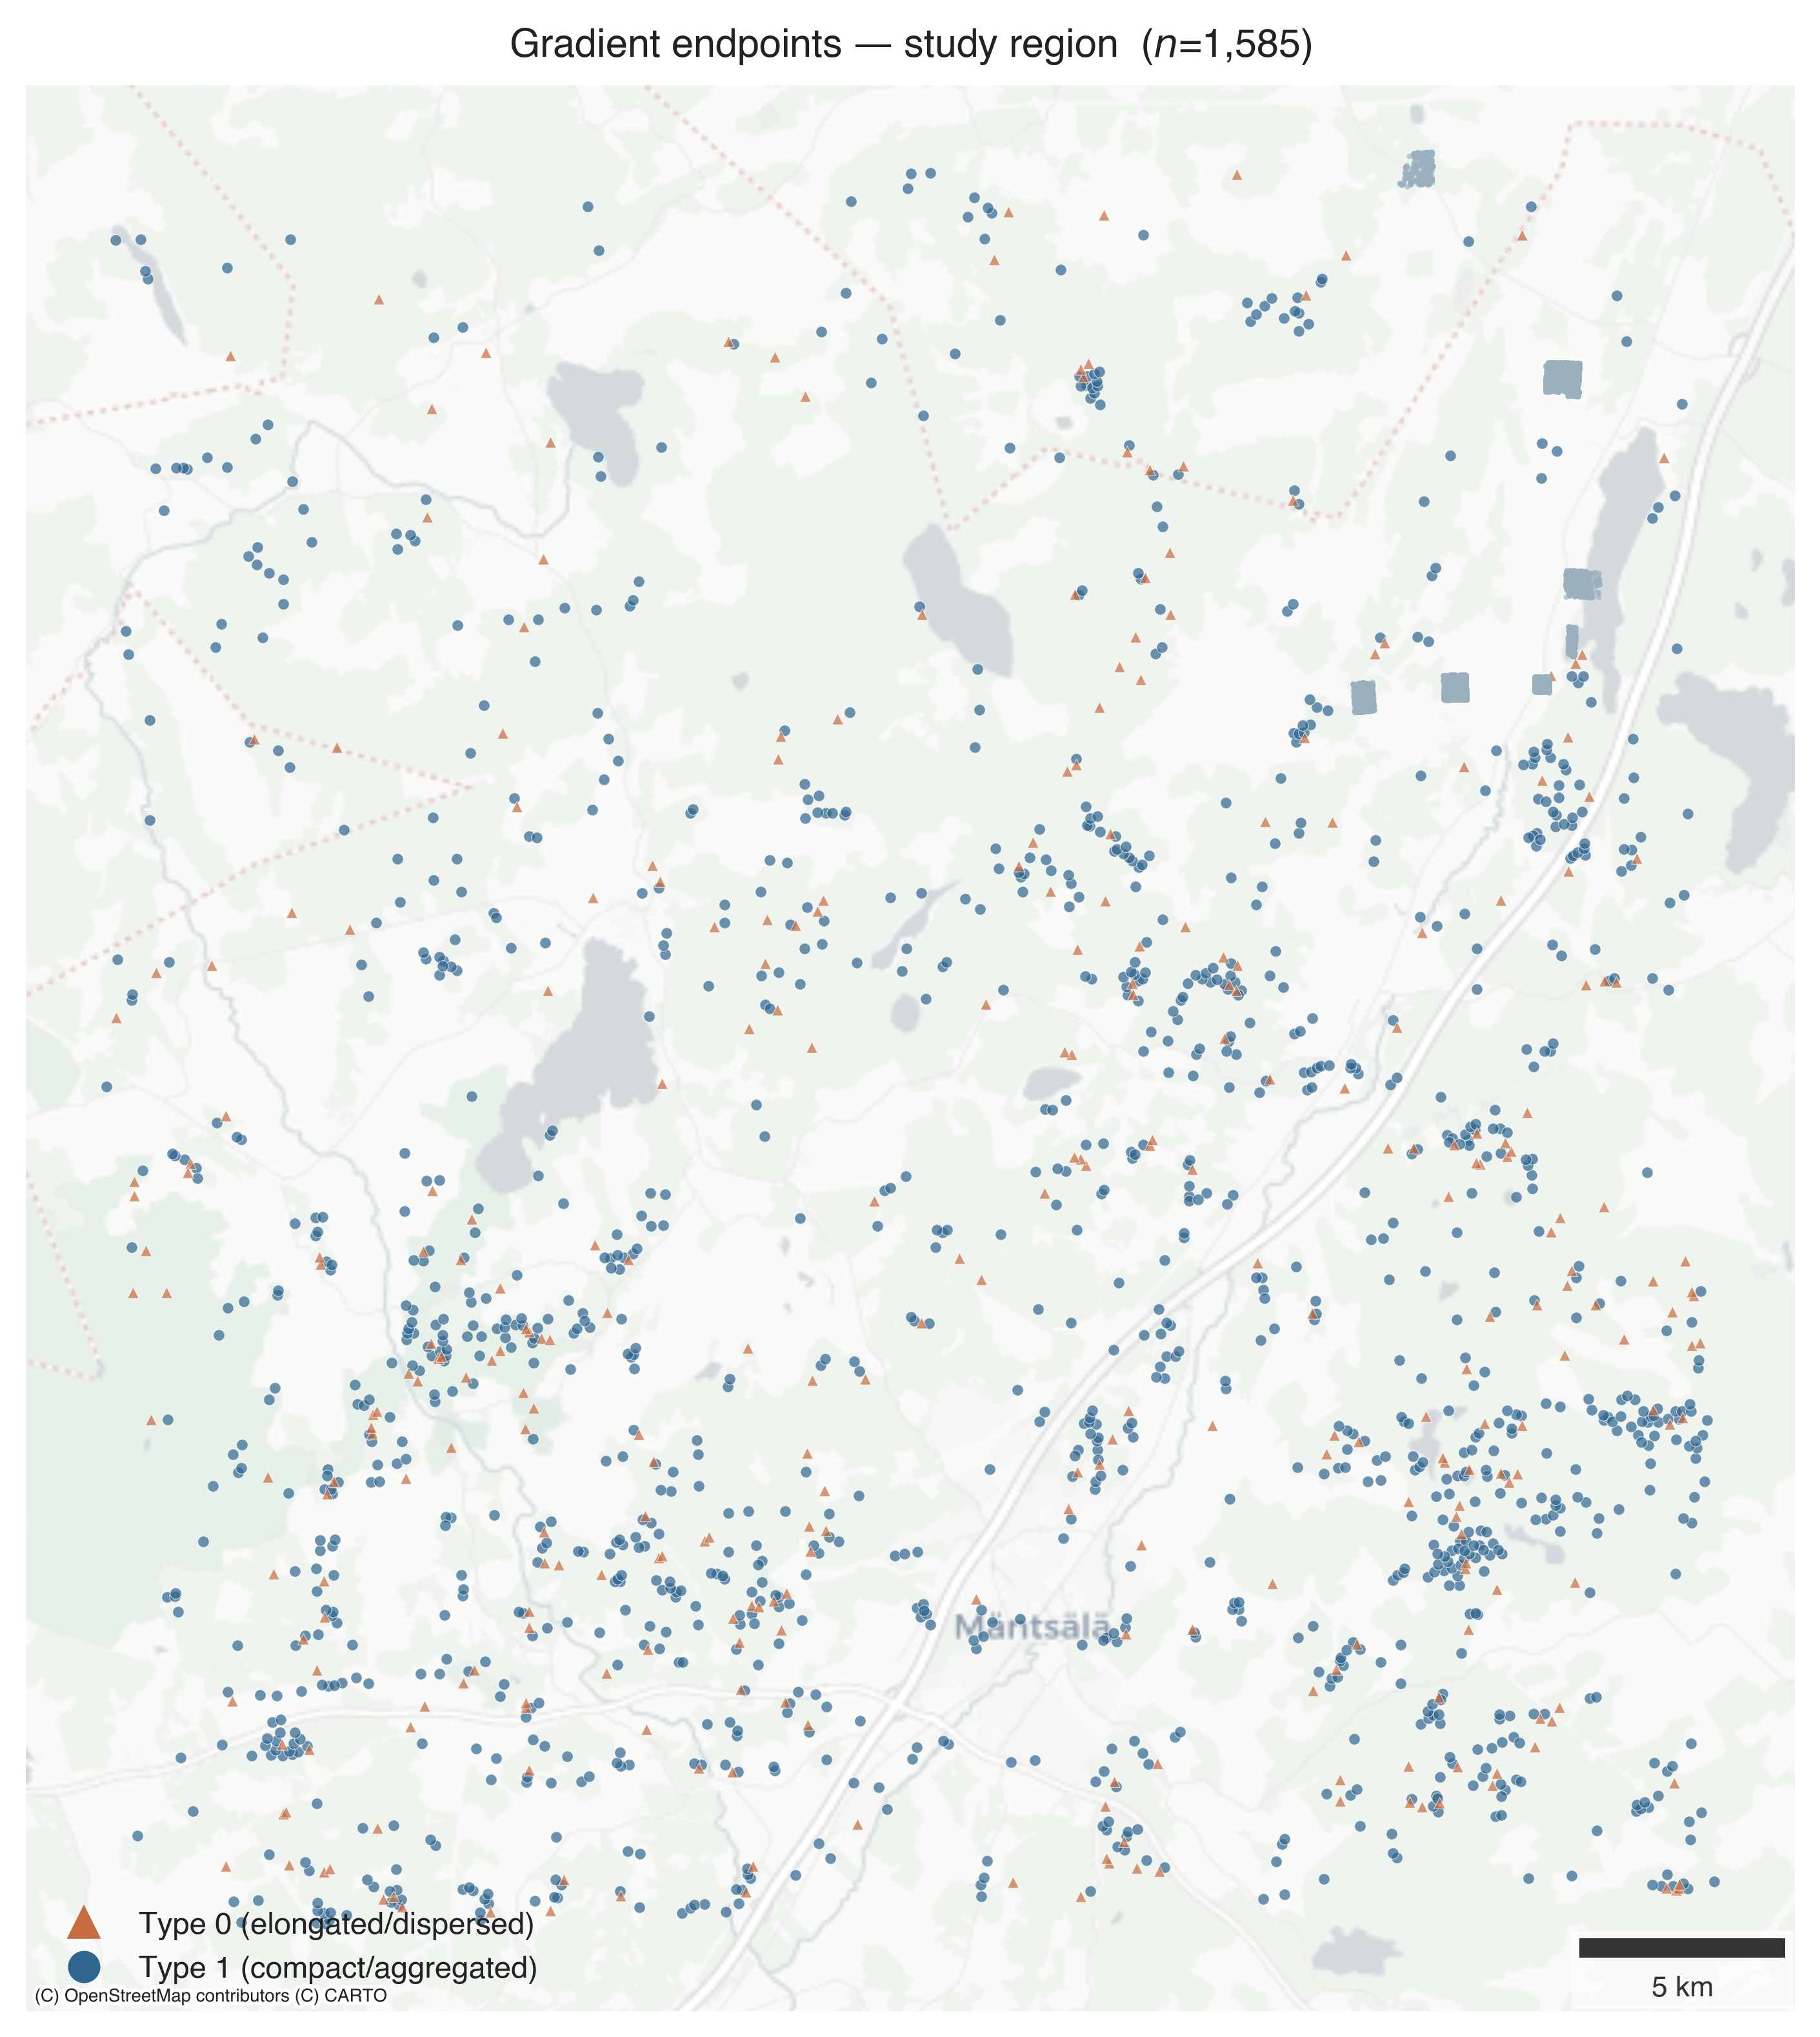
\includegraphics[width=0.9\linewidth]{fig6_typology_map.png}
  \caption{Spatial distribution of the two gradient endpoints within a southern display window
           (one tile, 10.9\% of clusters, shown for legibility). Blue circles: Type\,1
           (compact/aggregated); brown triangles: Type\,0 (elongated/dispersed). Inset: all 14,582
           clusters sampled across Finland for geographic context.}
  \label{fig:typology_map}
\end{figure}

\begin{figure}[htb]
  \centering
  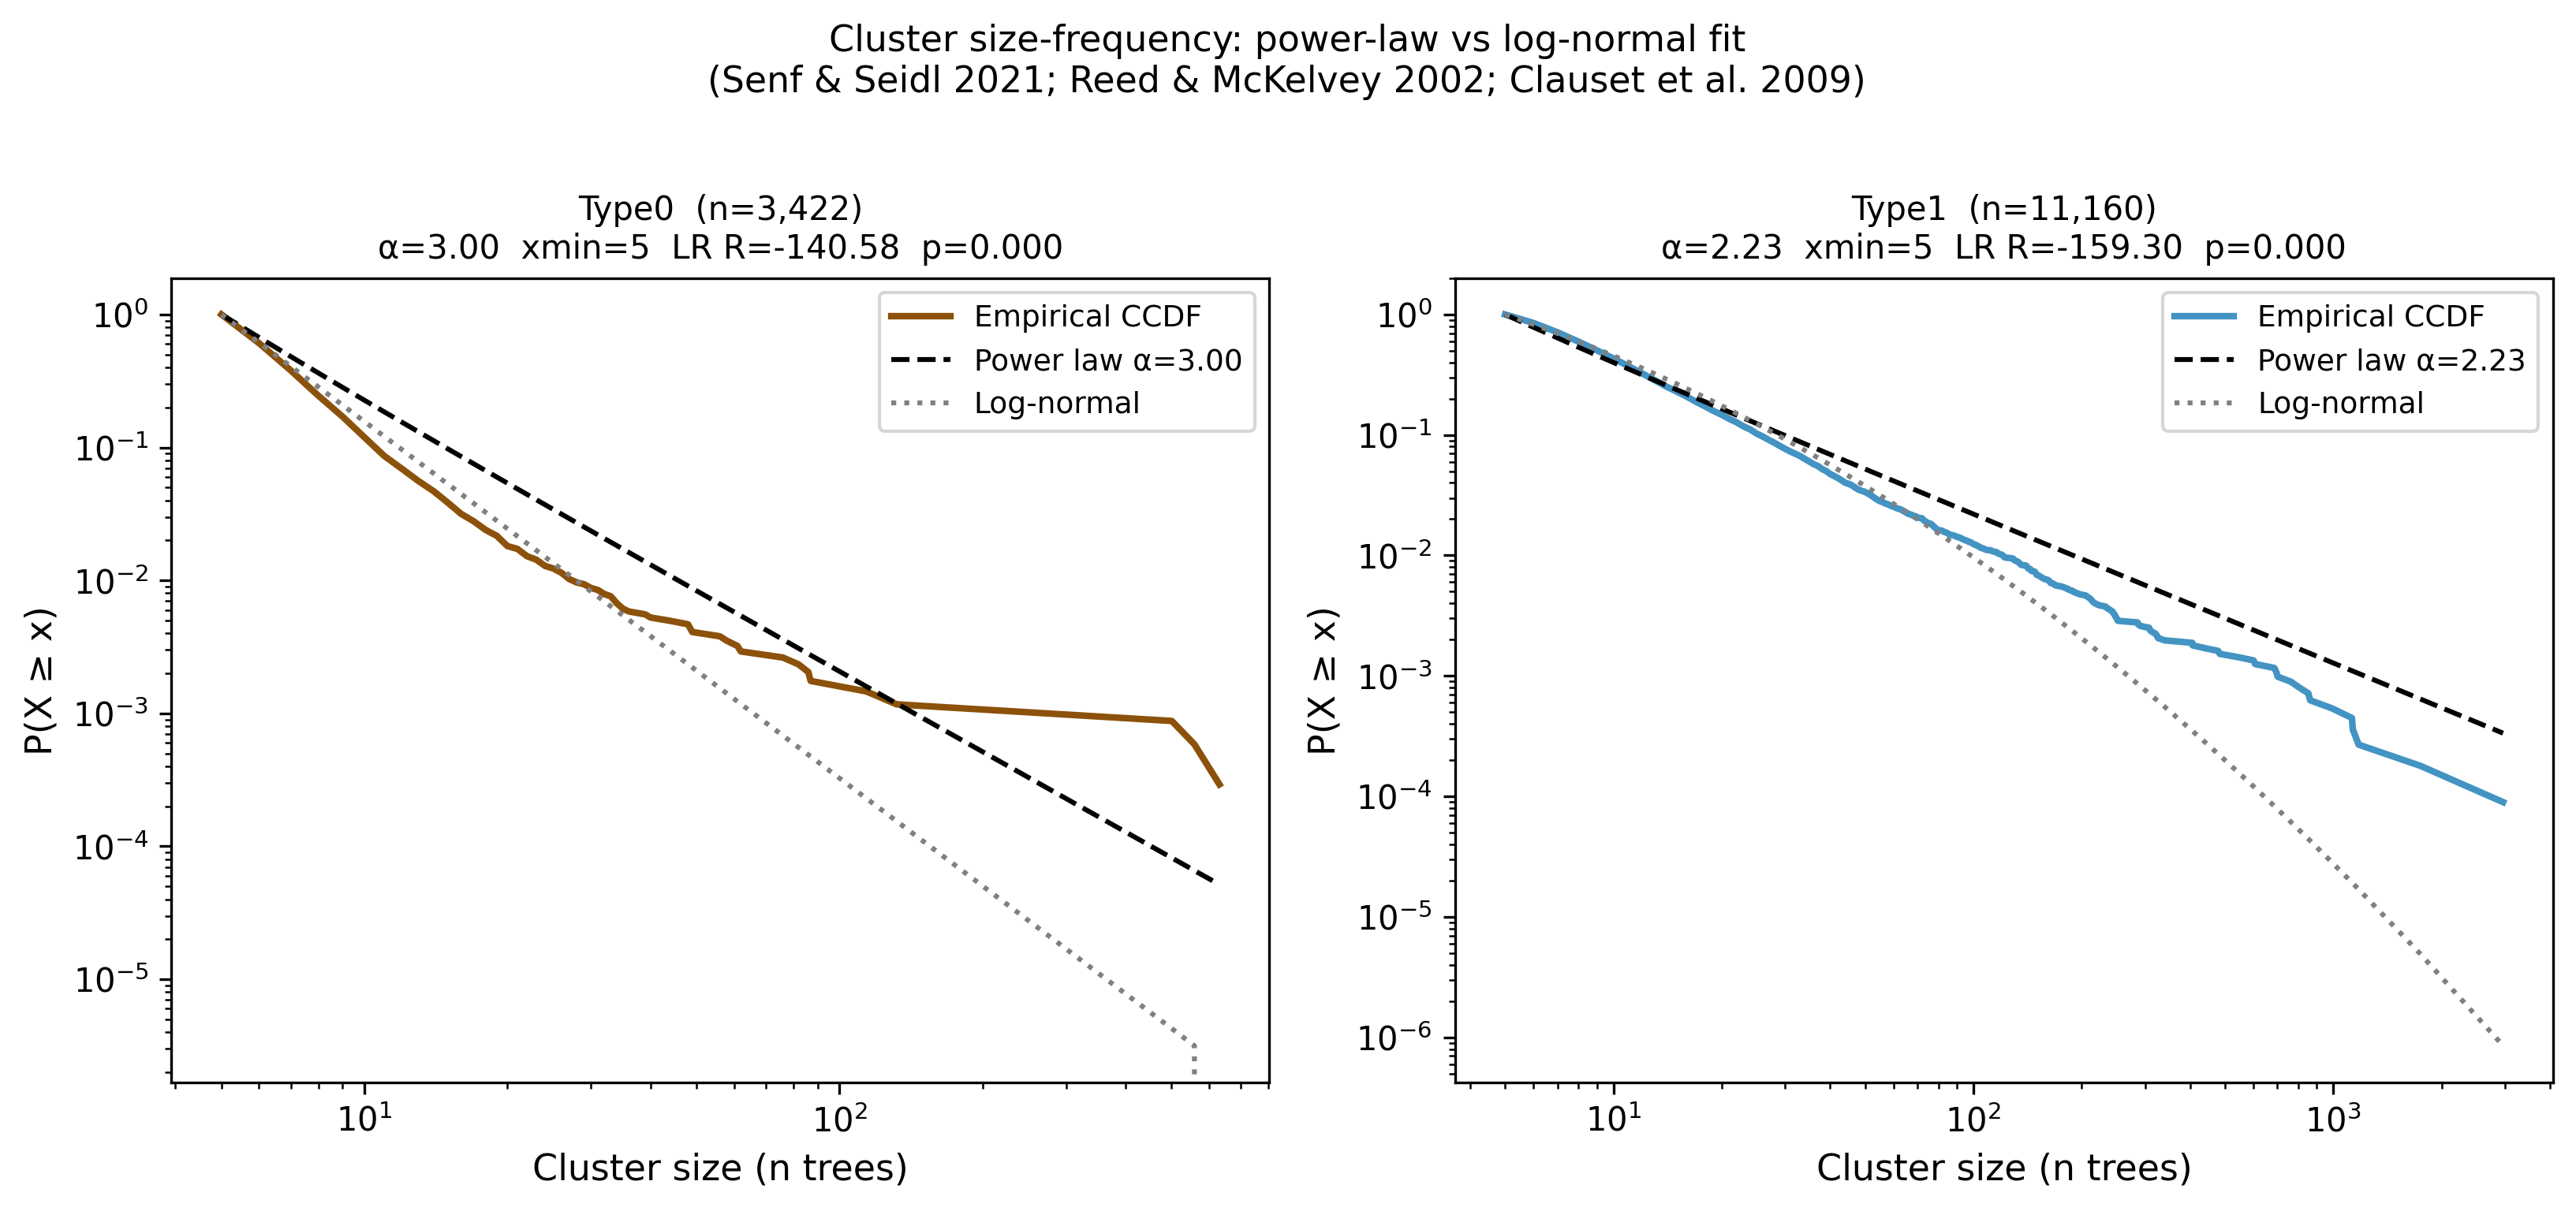
\includegraphics[width=0.9\linewidth]{fig_size_dist.png}
  \caption{Complementary cumulative distribution functions (CCDF) of cluster size ($n$) per endpoint.
           Both are better described by a lognormal than a power law; Type\,1 has the heavier upper
           tail, consistent with its larger mean cluster area.}
  \label{fig:sizedist}
\end{figure}

\begin{figure}[htb]
  \centering
  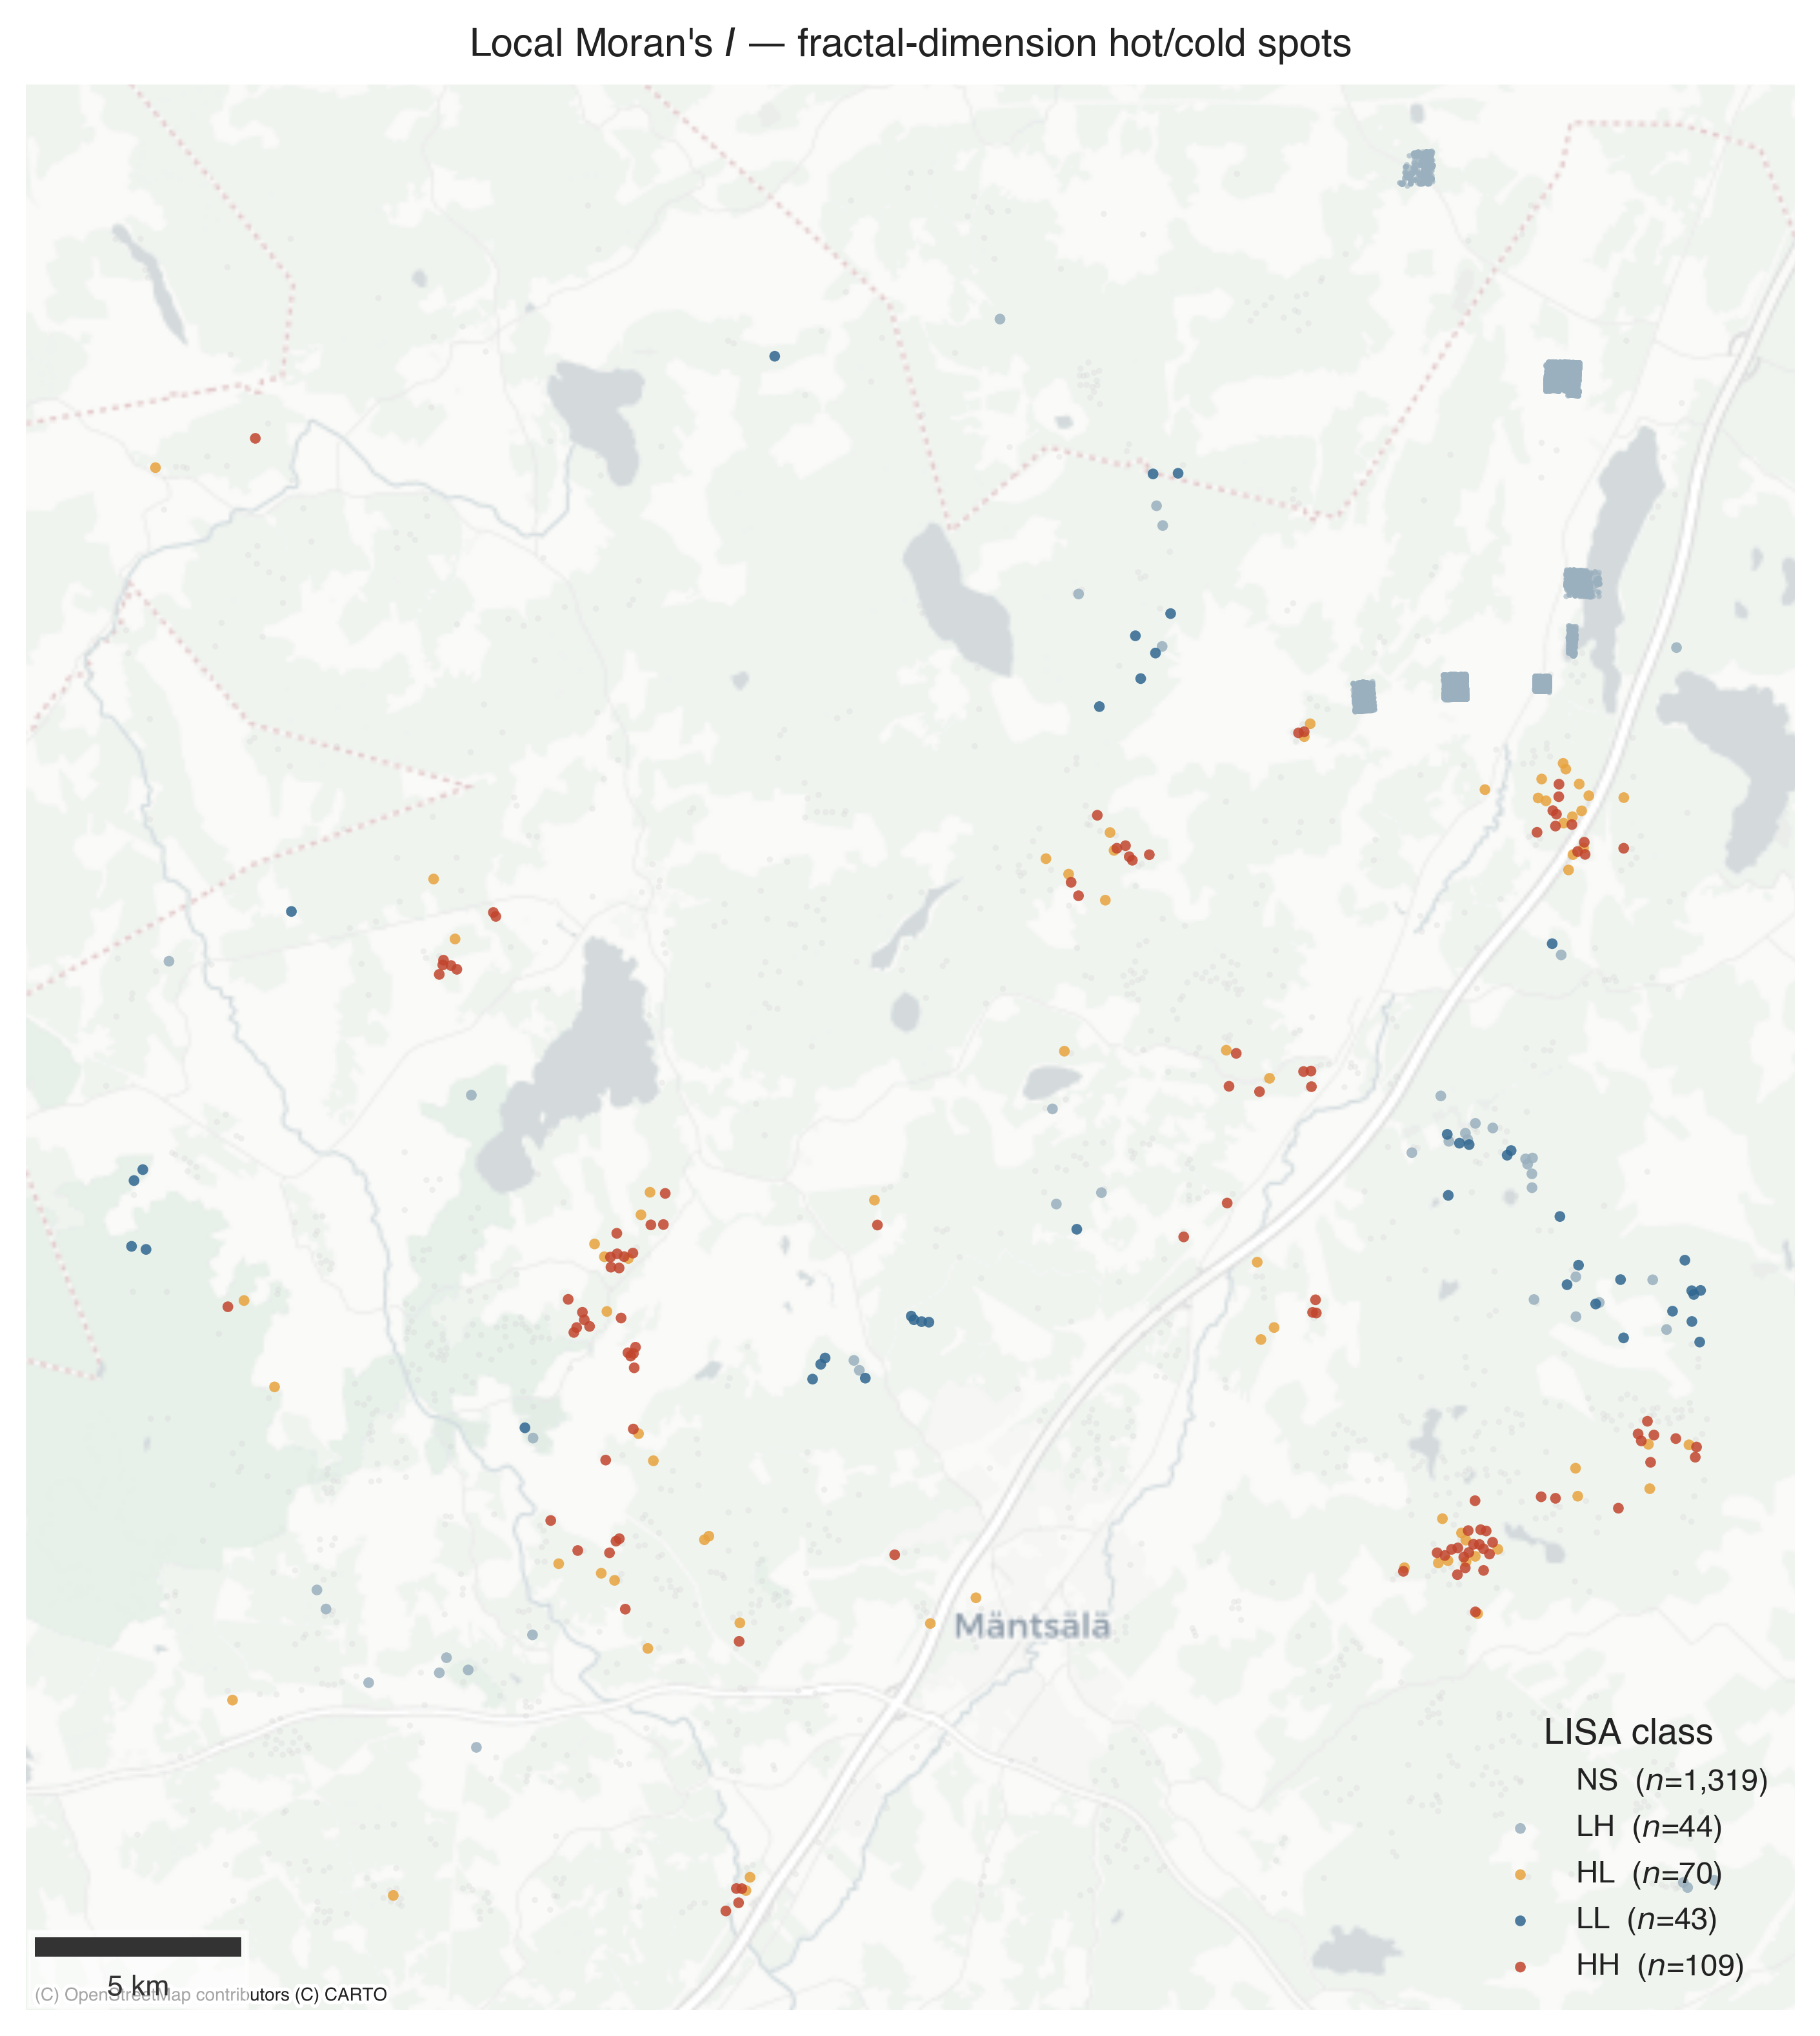
\includegraphics[width=0.9\linewidth]{fig8_local_morans.png}
  \caption{LISA hotspot map for fractal dimension in the southern display window. Labels computed on
           the full survey dataset. Red: high--high clusters; blue: low--low clusters. Inset:
           full-survey cluster distribution for geographic context.}
  \label{fig:lisa}
\end{figure}

\begin{figure}[htb]
  \centering
  \begin{subfigure}{0.9\linewidth}
    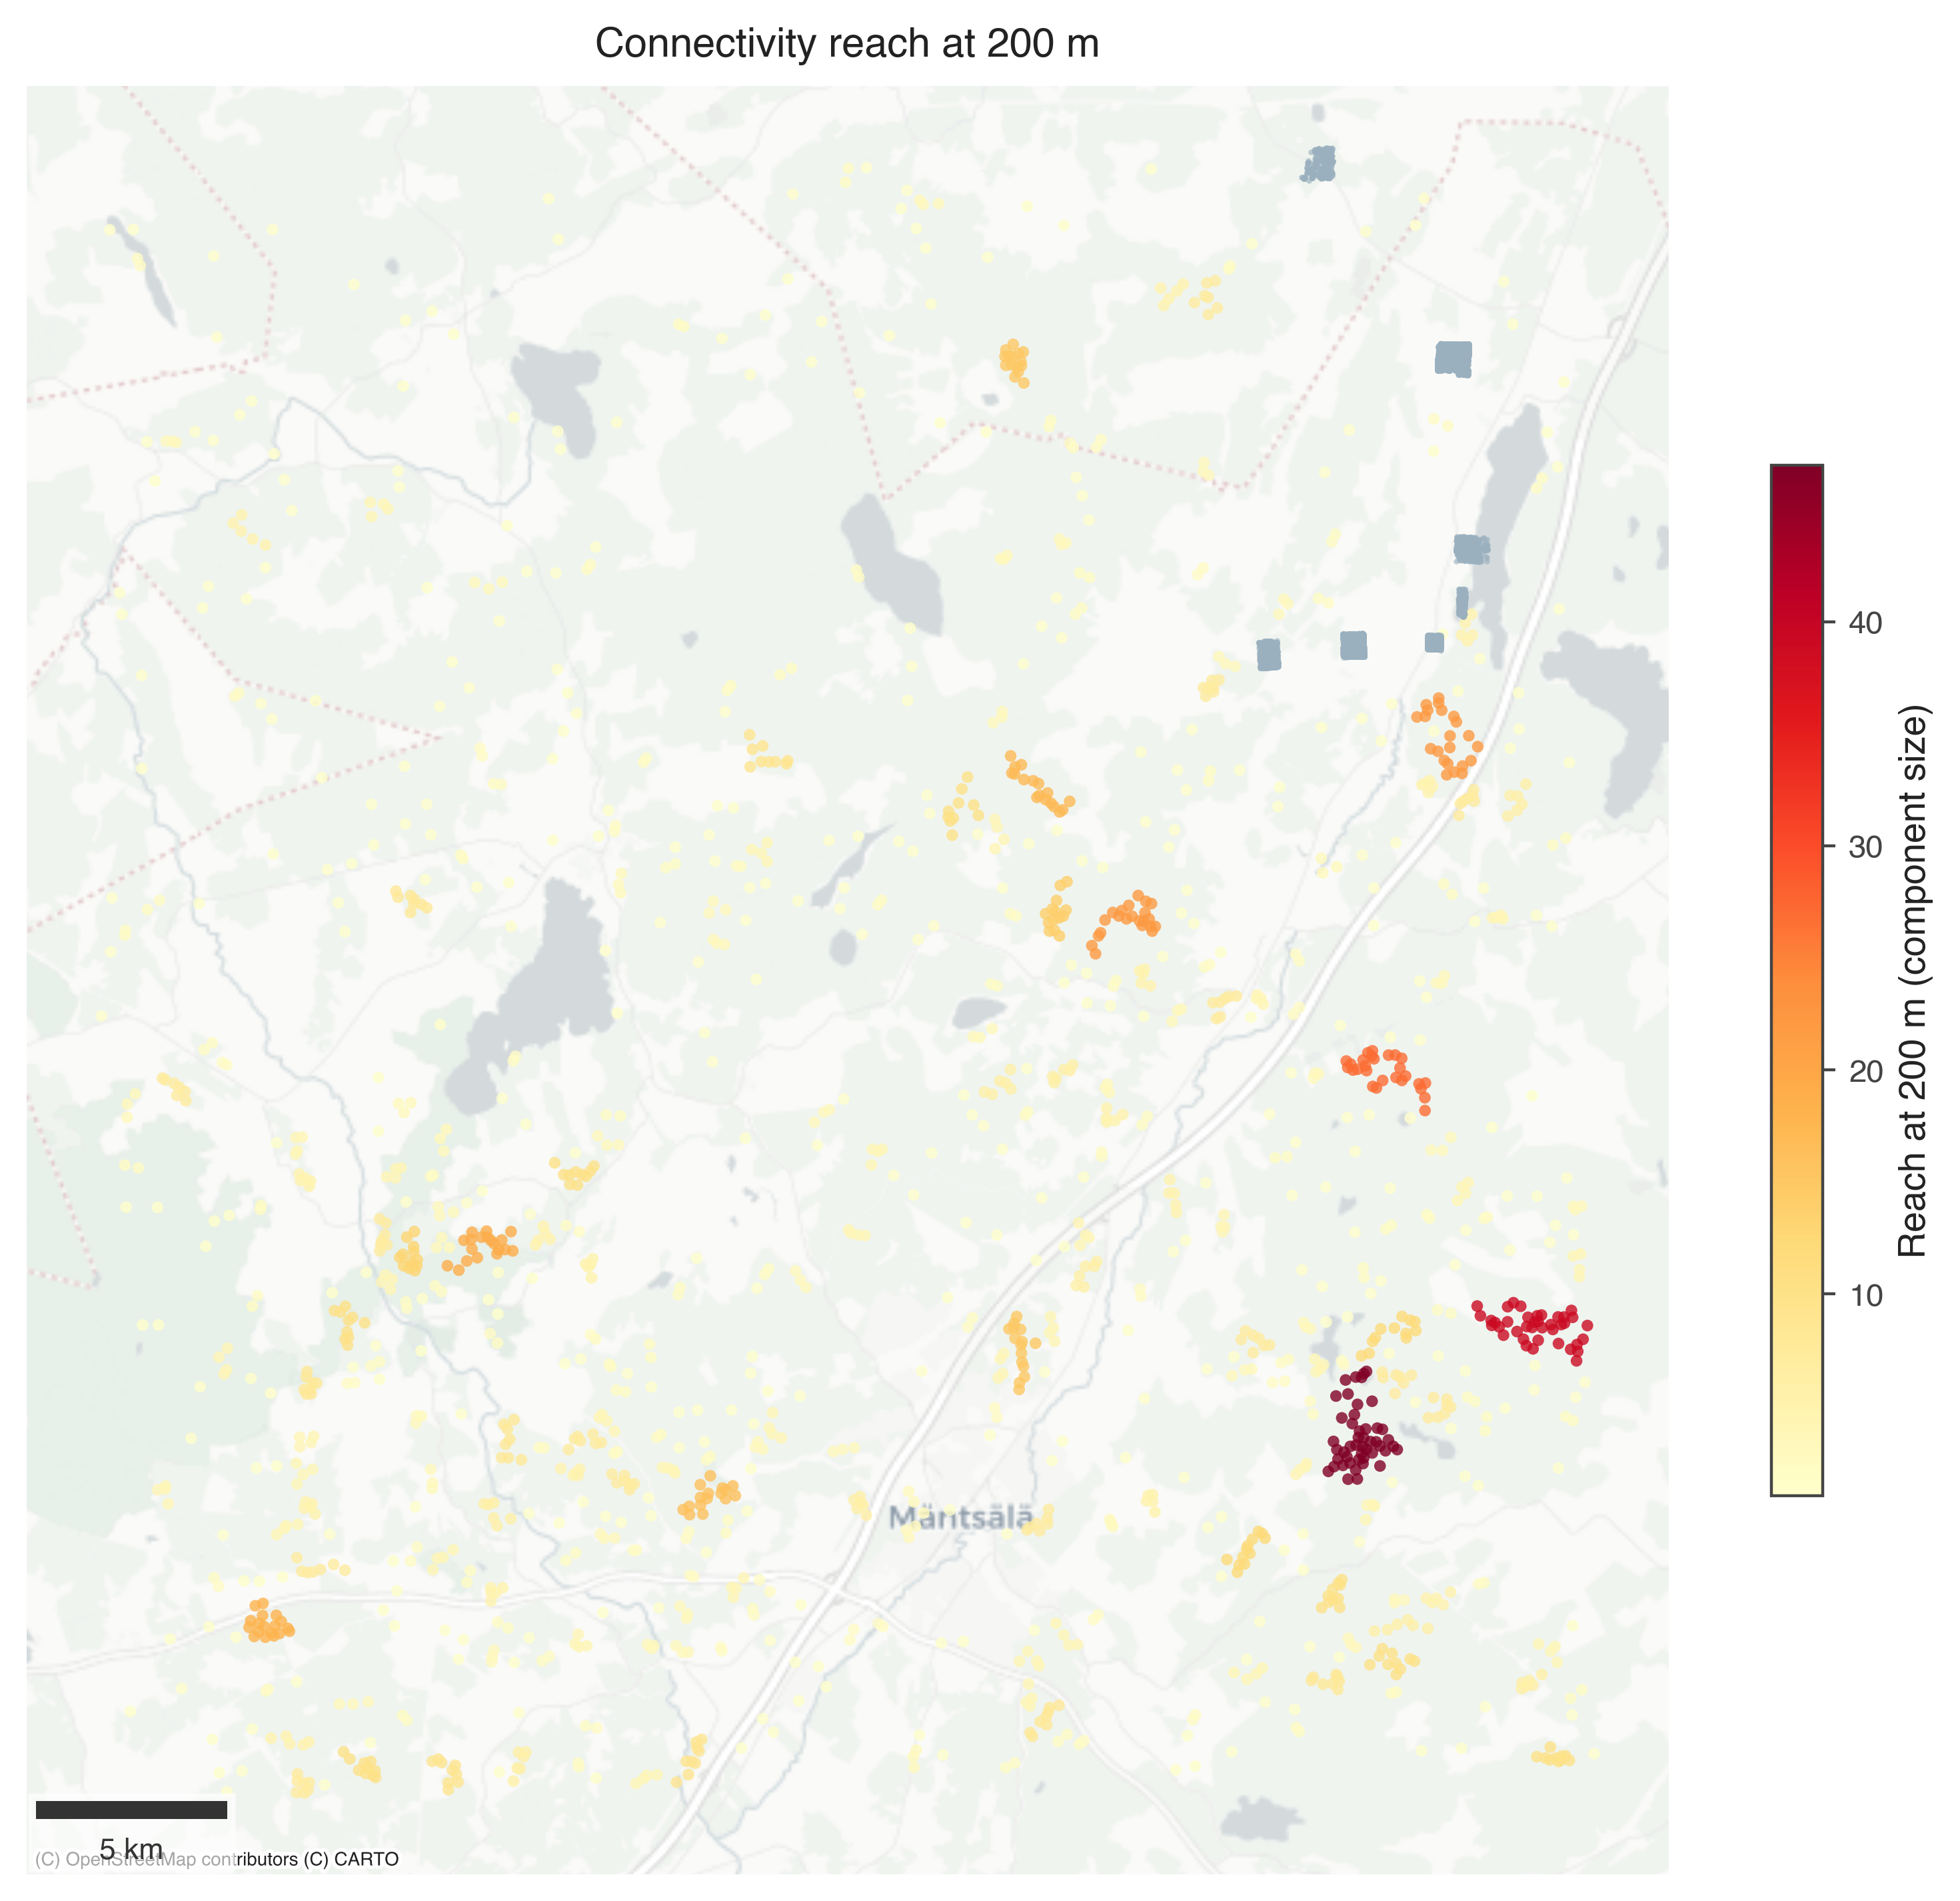
\includegraphics[width=\linewidth]{fig_contagion_a.png}
    \caption{Connectivity reach at 200\,m (component size). Inset: full-survey cluster distribution.}
    \label{fig:contagion_a}
  \end{subfigure}
  \begin{subfigure}{0.9\linewidth}
    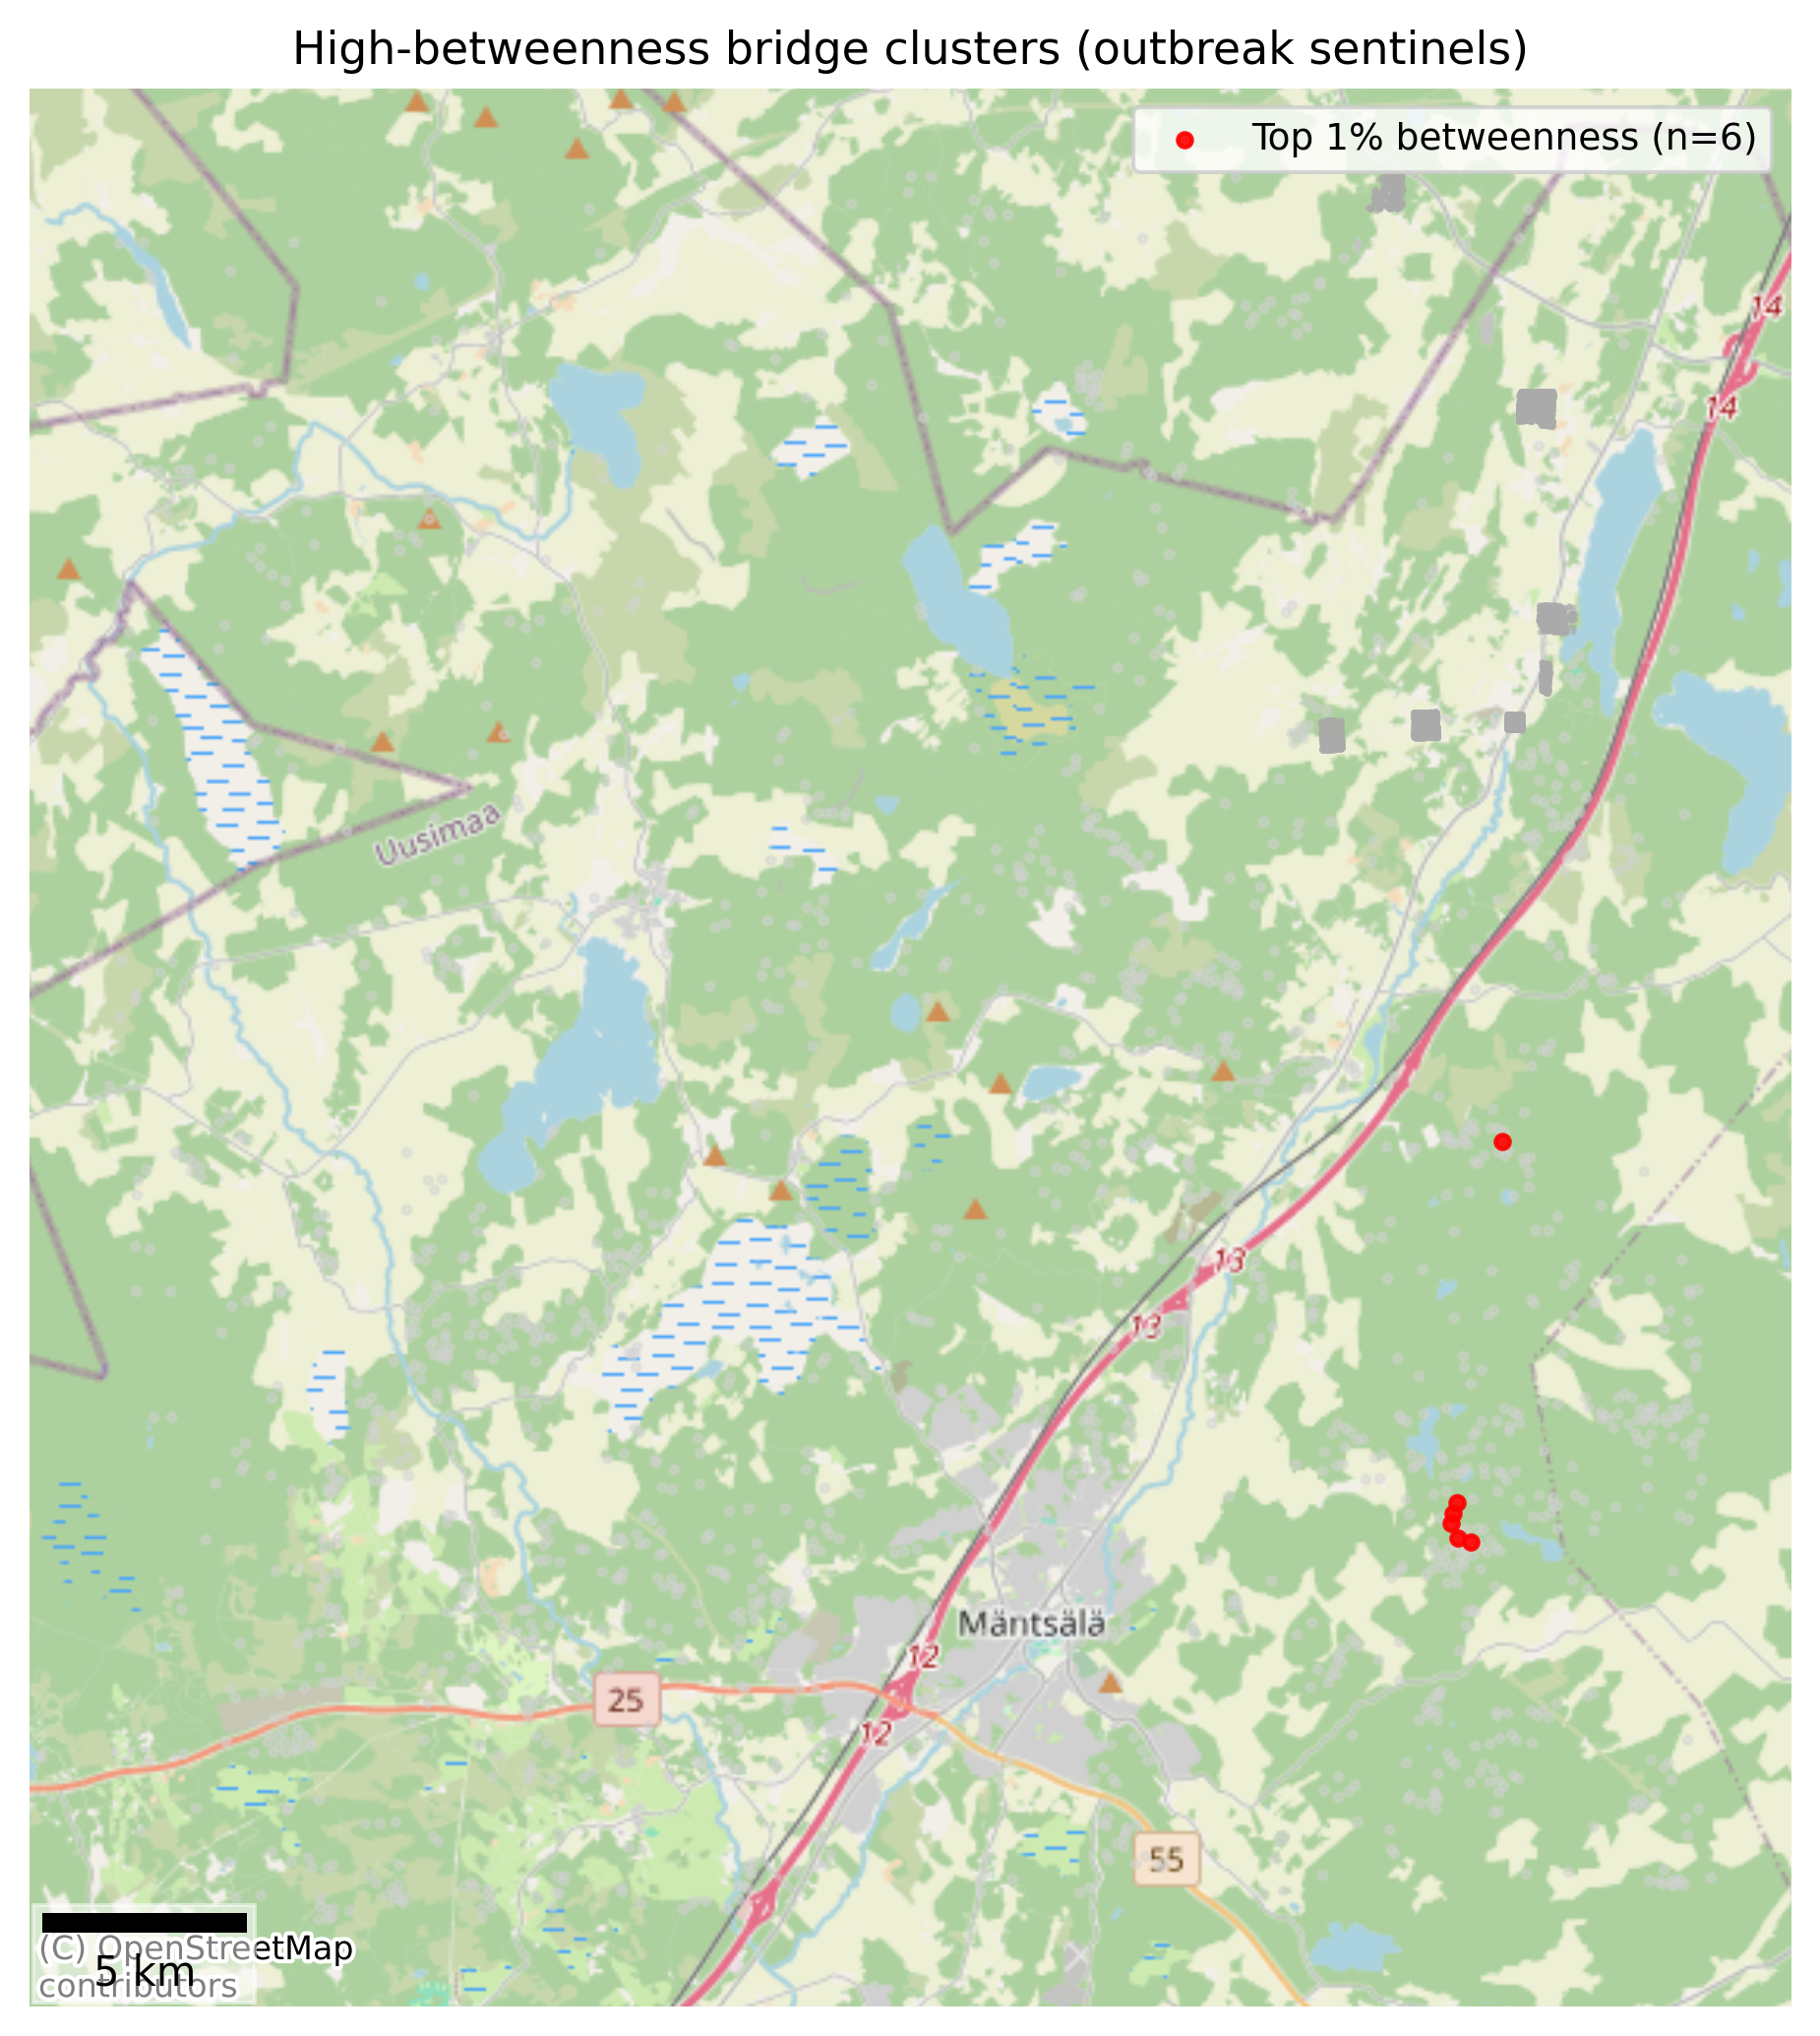
\includegraphics[width=\linewidth]{fig_contagion_b.png}
    \caption{Top 1\% betweenness clusters (red) as geometric articulation points (no temporal
             validation). All metrics computed on the full graph.}
    \label{fig:contagion_b}
  \end{subfigure}
  \caption{Landscape connectivity in the southern display window.}
  \label{fig:contagion}
\end{figure}

\begin{figure}[htb]
  \centering
  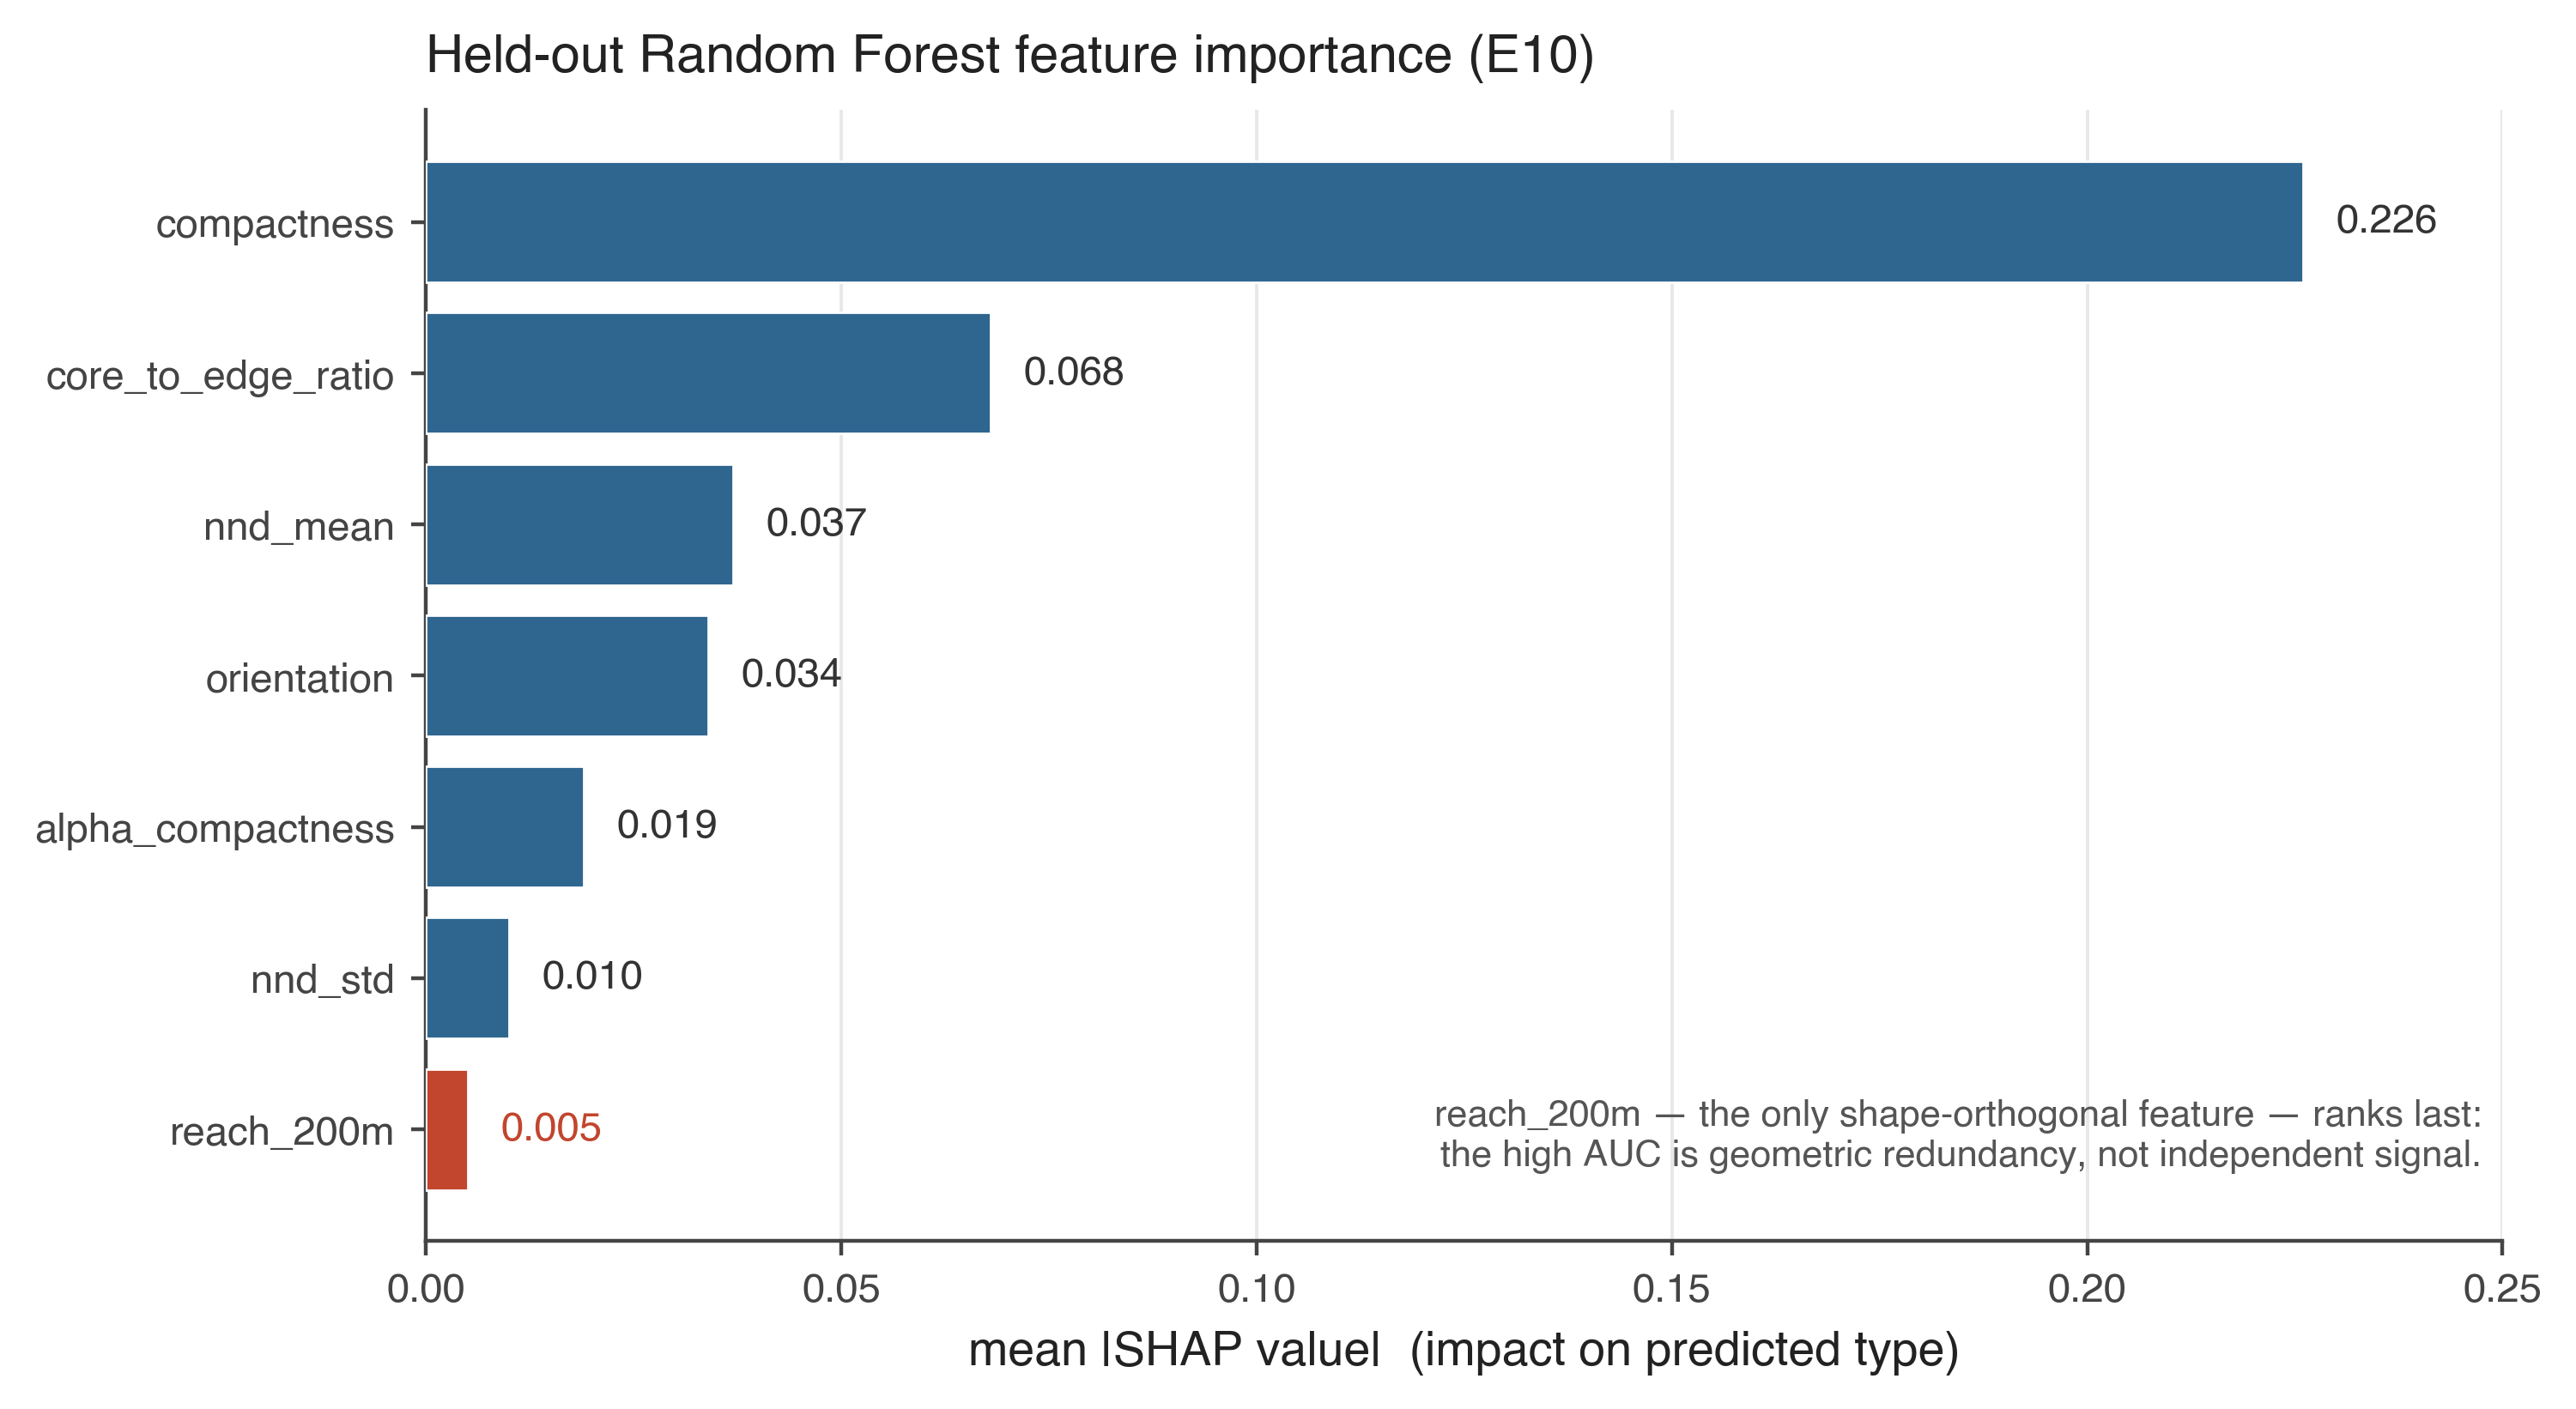
\includegraphics[width=0.9\linewidth]{fig_shap_heldout.png}
  \caption{Mean $|$SHAP$|$ feature importance for the held-out Random Forest. Compactness dominates;
           reach\_200m (the only shape-orthogonal feature, highlighted) ranks last, so the high AUC
           reflects geometric redundancy among shape descriptors rather than independent signal.}
  \label{fig:shap}
\end{figure}

\end{document}
